\subsection{Handling invalid data in real-time}
\label{sec:data_issues}

Much of the degeneration or \emph{vehicle loss} can be attributed to irregularities with the incoming real-time data. There are two leading causes of this, described below, which can be detected and potentially avoided with a similar solution.


\paragraph{Buses that appear to go backwards}

One of the prominent assumptions of our model is that the bus cannot go backwards along the route, which is implemented by only allowing for non-negative values of speed. However, a couple of scenarios can lead to the \emph{appearance} of a reversing bus, both of which are related to \emph{\gls{gps} waypoints}; that is, the \gls{avl} systems in Auckland Transport's buses are programmed to not only report their position periodically but also to report their arrival at certain waypoints. These can include bus stops (which result in an arrival or departure time update) as well as some major intersections. The issue is that, rather than reporting the bus's \gls{gps} position, they report the \gls{gps} coordinates of the waypoint itself. This is often acceptable since the bus continues straight past the intersection or bus stop before reporting another position. However, if there is congestion leading into the waypoint, the bus may:
\begin{enumerate}[i.]
\item approach the waypoint, decide it has arrived, and report its position \emph{at the waypoint},
\item get stopped in a queue for some time,
\item decide it is time for another position update, based on its GPS position.
\end{enumerate}
\Cref{fig:bus_going_backwards} presents an example of this.

\begin{knitrout}\small
\definecolor{shadecolor}{rgb}{0.969, 0.969, 0.969}\color{fgcolor}\begin{figure}

{\centering 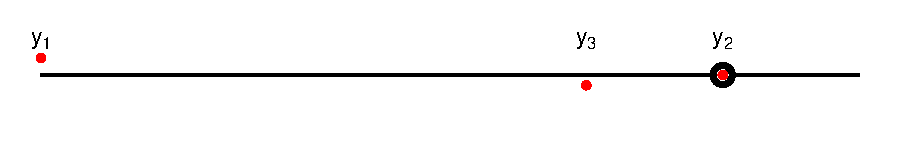
\includegraphics[width=.8\textwidth]{figure/bus_going_backwards-1} 

}

\caption[Three sequential observations of a vehicle approaching an intersection (hollow circle)]{Three sequential observations of a vehicle approaching an intersection (hollow circle). When the bus nears the intersection, it reports its position exactly at the intersection ($\Vobs_2$); however, there is a queue at this intersection, so the next observation ($\Vobs_3$) is behind the previous one, which gives the bus the appearance of going backwards.}\label{fig:bus_going_backwards}
\end{figure}


\end{knitrout}


The effect this has on the \pf{} is that, after observing $\Vobs_2$, the vehicle's state (represented by a sample of particles) will all be around the intersection. On receiving the next observation $\Vobs_3$, the particles are transitioned \emph{forward} by $(\Vtime_3 - \Vtime_2)$~seconds, which places them at or beyond the intersection; none of the particles will be near observation $\Vobs_3$ and will likely all have a likelihood of zero. In this case, the particle filter has degenerated and needs reinitialising.


A similar situation occurs when approaching a bus stop that has an intersection just before it. Here, the bus gets stopped at the intersection, but not before reporting its position at the stop since it was almost there. A subsequent observation then shows the bus at the intersection, which again appears to involve a reversing bus. The main issue we face is that \emph{we do not know the location of intersections} since there is no easily accessible data for this.\footnote{We presented an intersection model, but this was more of a demonstration of flexibility, not of functionality.}


Checking for the bus-reversing scenario in real-time requires mapping of observations onto the route shape; that is, the \emph{inverse measurement function}, allowing us to detect if the bus has gone backwards:
\begin{equation}
\label{eq:vehicle_rev_check}
\Vmeas^{-1}(\Vobs_k) < \Vmeas^{-1}(\Vobs_{k-1}).
\end{equation}
Of course, the inverse function is not exact, since the true location is unlikely to be positioned exactly on the line (roads have width, and \gls{gps} devices have error). To compute $\Vmeas^{-1}$, we find the shortest distance along the route's shape that is closer than a threshold of $3\GPSerr$, which allows for situations where the route passes the observed location point more than once (such as in loops).

If the observation is determined to be going backwards, we have to decide between
\begin{enumerate}[i.]
\item ignoring the current observation, or
\item ignoring the previous observation and restoring the vehicle's previous state.
\end{enumerate}
If we can determine that the first observation is a pre-emptive observation (that is, at a waypoint), then option (ii) is the logical choice, although this requires storing each vehicle's state \emph{twice}. Otherwise, it is easier to ignore the current observation completely and use option (i). Note that, were intersection locations knowable, we could include this behaviour in the model; as it stands, however, this workaround is required to avoid unnecessary degeneration.


\paragraph{Buses that remain stationary}

Another situation (which can also occur around unknown intersections) is when the bus does not move between successive observations (or it moves very slowly). For example, the bus may need to turn onto a major road, for which there is a queue of traffic. The bus will report its position when it arrives, and may again report its position after moving a few meters. If our model does not allow for the bus to suddenly slow down in these situations, the particles will all be far ahead of the bus and degeneration will occur.


We can determine if the bus has remained more-or-less stationary by computing the distance between successive observations and comparing to a threshold:
\begin{equation}
\label{eq:vehicle_dist_check}
\dist{\Vobs_{k-1}, \Vobs_k} < \distThreshold =
\Vtdiff_k \min_i\left(\Vspeed_k\vi\right)
\end{equation}
The threshold here is the expected distance travelled in $\Vtdiff_k$~seconds by the slowest particle. Rather than slowing the particles (which could run into the opposite problem once the vehicle passes through the intersection), we sample a temporary speed
\begin{equation}
\label{eq:vehicle_temp_speed}
\Vspeed_k\vi \sim
\Uniform{0}{\frac{\dist{\Vobs_{k-1}, \Vobs_k}}{\Vtdiff_k}}
\end{equation}
which is used for one single iteration.

Again, if we knew the locations of intersections, we could integrate this behaviour into the model. Particles could partake in ``creeping'' up to the intersection, before quickly accelerating back up to speed on the next road segment. Even then, however, the above behaviour would still need to be included to handle non-intersection related slowing down, for example, when reaching a congested section of a road.
